\documentclass{beamer}
\usepackage[utf8]{inputenc}
\usepackage{graphicx}
\usepackage{url}

\author[Sowmya Vajjala]{Instructor: Sowmya Vajjala}


\title[LING 120]{LING 120: \\ Language and Computers}
\subtitle{Semester: Fall '17}

\date{30 October 2017}

\institute{Iowa State University, USA}

%%%%%%%%%%%%%%%%%%%%%%%%%%%

\begin{document}

\begin{frame}\titlepage
\end{frame}

\begin{frame}
\frametitle{Today's topic}
\begin{center}
\Large How are dialog systems and chat bots made?
\tiny \\
(Materials from: Textbook, and "Speech and language processing" by Jurafsky and Martin (Chapters 29--30))
\end{center}
\end{frame}

\begin{frame}
\frametitle{on Eliza - some comments from your responses}
\begin{itemize}
\item "The bot mostly just tries to identify parts of your sentence and parrot them back to you in the form of a question. Which I suppose is the idea behind the stereotypical therapist"
\item "However if you dig too deep, use sarcasm or modern slang it doesn't really understand so it'll ask very broad open questions."
\item "This bot isn't very good at relying on context."
\item "My overall evaluation of the program is that it does a decent job of fulfilling the role of a psychoanalyst, however, it is clearly built on a certain structure with only a handful of cases."
\end{itemize}
\end{frame}

\begin{frame}
\frametitle{on Siri - some comments from your responses}
\begin{itemize}
\item can interpret that 9 and nine are same, "having a meeting" is about scheduling etc, but cannot identify am vs pm.
\item Cannot identify that "language and computers" is one entity, and hence shows two search results.
\item Better with specific questions, but not at general talk
\item Speech recognition is not perfect.
\end{itemize}
\end{frame}

\begin{frame}
\frametitle{Summary of the responses}
\begin{itemize}
\item Eliza seems to be bad at general chatting, but does some specific kinds of chats well.
\item Siri is also good with certain things (doing specific tasks) but not good with conversations.
\item Eliza is 50 years old. Siri is latest - yet, some issues persist.
\item Does it mean these dialog systems are no good even now? \pause
\item Clearly, recent technological developments enabled chat bots that do specific tasks do well (morph.ai etc from last class)
\end{itemize}
\end{frame}

\begin{frame}
\frametitle{What we should take care of when automating dialog-0}
What are some of tasks that come to your mind if someone asks you to make something like Siri? 
\end{frame}

\begin{frame}
\frametitle{What we should take care of when automating dialog-1}
\begin{itemize}
\item Study the purpose
\item Understand the users
\item What sort of interaction will happen? (text or speech or both?)
\item Build simulations and prototypes (Wizard of Oz simulations)
\item Iteratively test the design on real users and get feedback.
\end{itemize}
\end{frame}

\begin{frame}
\frametitle{What we should take care of when automating dialog-2}
\begin{itemize}
\item Starting a conversation (Who starts? User or System? How?)
\item Understanding what the user said (question? request? general statement?)
\item Formulating appropriate response
\item Learning when to stop/how to stop the conversation
\item Keeping track of the dialog
\end{itemize}
\end{frame}

\begin{frame}
\frametitle{Types of Dialog Systems}
\begin{itemize}
\item Rules and pattern-matching based (e.g., Eliza) - typically use regular expressions.
\item Frame-based dialog agents (e.g., flight booking systems, LetsGo etc) - focused on specific tasks 
\item Retrieval based (e.g., FAQ bots) - they mine large datasets of human conversations to map from user to system response.
\item Latest research in this direction uses something called sequence-to-sequence neural networks.
\end{itemize}
\end{frame}

\begin{frame}
\frametitle{Rule-based: How does Eliza Work?}
\begin{itemize}
\item As some of you already noticed, Eliza is based on matching keywords in your text. 
\item Its responses are based on a series of regular expressions. 
\item one version of Eliza, written in Python: \url{https://github.com/jezhiggins/eliza.py}
\item This will really work, sometimes. Some people also got attached to Eliza.
\end{itemize}
\end{frame}

\begin{frame}
\frametitle{Rule-based: Parry}
\begin{itemize}
\item another chat-bot with a psychology focus: to study schizophrenia.
\item In addition to patterns, like Eliza, Parry has an additional variable: mental states. Certain topics change Parry's emotional state!
\item Parry was known to pass a version of the "Turing Test" in 1972!!
\item More at: \url{https://en.wikipedia.org/wiki/PARRY}
\item Parry meets Eliza: \url{https://phrasee.co/parry-the-a-i-chatterbot-from-1972/}
\end{itemize}
\end{frame}

\begin{frame}
\frametitle{Frame based dialog agents}
\begin{itemize}
\item Dialog systems with very specific goals (e.g., LetsGo system we saw last week from CMU).
\item All communication is seen as coming from a set of "frames" with vacant "slots" that need to be filled with "values" based on human responses. 
\item A frame for LetsGo could be looking for the vacant slots for: Origin, Destination, Departure time, Arrival time, Departure date, Bus number. (\url{http://www.speech.cs.cmu.edu/letsgo/example.html})
\item Each slot can have a collection of questions, of which the system picks some to ask the user. 
\end{itemize}
\end{frame}

\begin{frame}
\frametitle{Frame based dialog agents}
\begin{itemize}
\item May be there is a hierarchy in these slots (e.g., fill the bus number after filling other slots).
\item System needs to keep track of conversation history (unlike Eliza).
\item Other tasks: each time a user says something, system needs to determine what slot-filling template needs to be filled, what is next? etc. 
\item Language processing involved: POS tagging, named entity recognition, and so on. 
\end{itemize}
\end{frame}

\begin{frame}
\frametitle{Example structure of a frame based dialog }
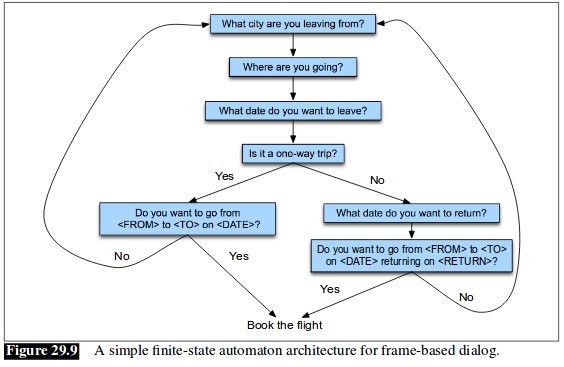
\includegraphics[width=0.9\textwidth]{framedialog.png}
\end{frame}

\begin{frame}
\frametitle{Retrieval Based agents}
\begin{itemize}
\item Instead of having specific patterns/rules, these rely on lots and lots of conversational, and question-answer data.
\item Like rule-based bots, focus is on responding to current statement, not tracking the history.
\item Bots can look online for answers to your questions (e.g., Siri) or in to their own pool of answers (morph.ai demos from last week)
\item You can combine this with a little bit of pattern matching, to add some "personality" to the bot (Siri)
\end{itemize}
\end{frame}

\begin{frame}
\frametitle{Dialog Acts - Understanding what user wants - Example 1}
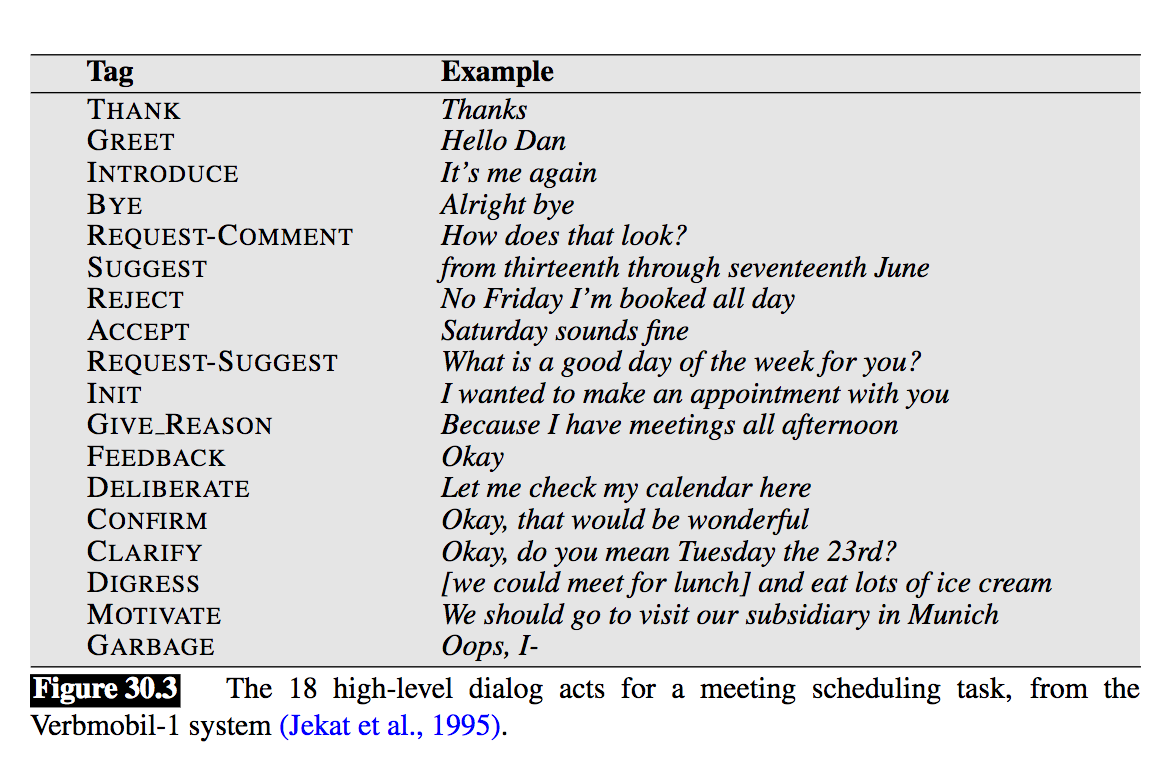
\includegraphics[width=0.9\textwidth]{dialogact1.png}
\end{frame}

\begin{frame}
\frametitle{Dialog Acts - Understanding what user wants - Example 2}
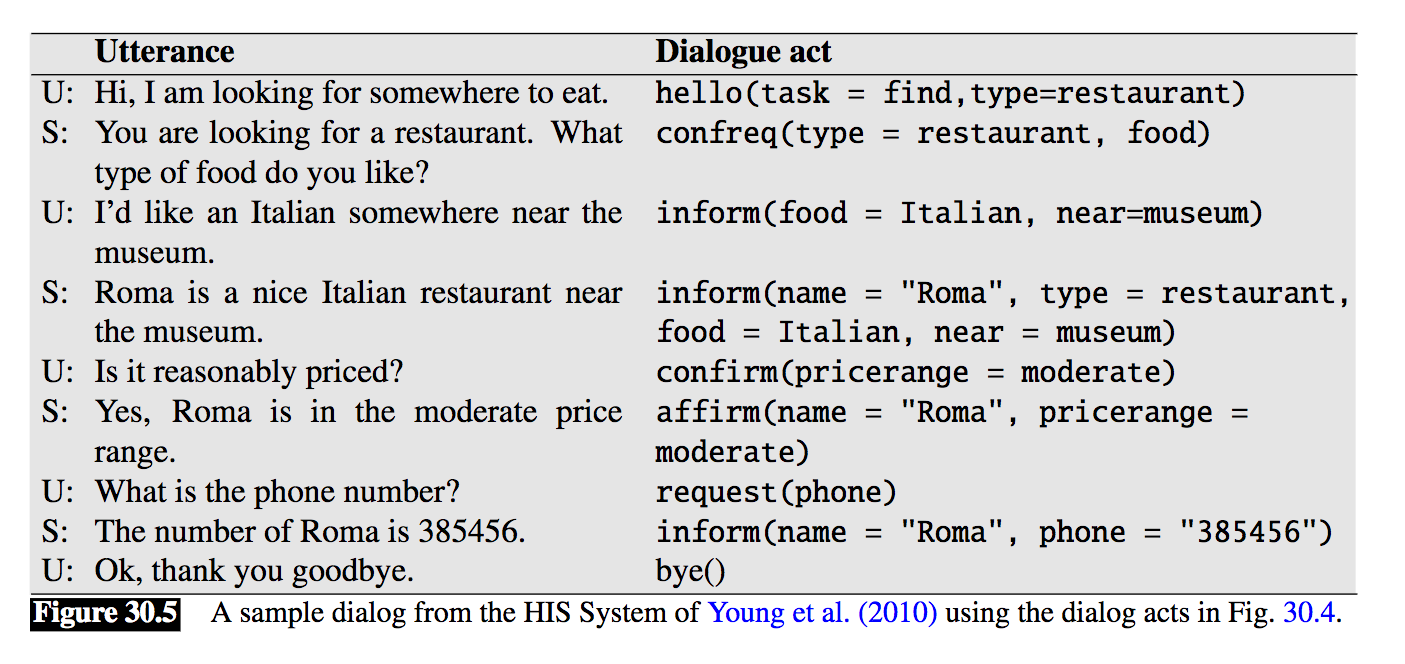
\includegraphics[width=0.9\textwidth]{dialogact2.png}
\end{frame}

\begin{frame}
\frametitle{Dialog Acts - Understanding what user wants - Example 3}
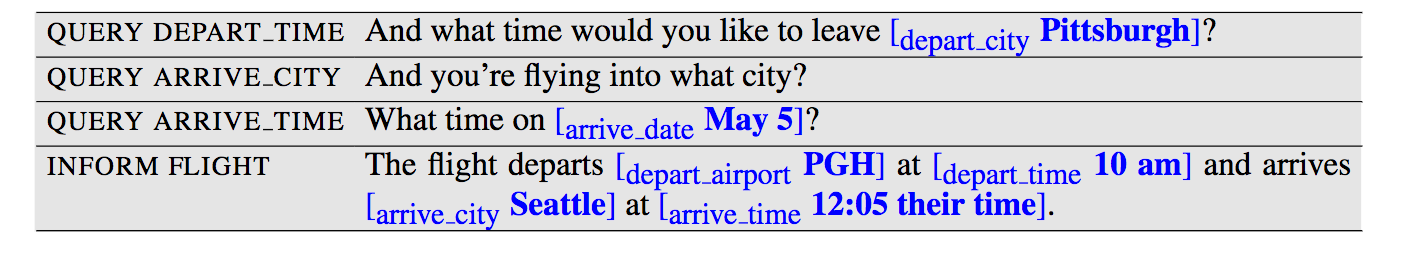
\includegraphics[width=0.9\textwidth]{dialogact3.png}
\end{frame}

\begin{frame}
\frametitle{General Links}
\begin{itemize}
\item Humor: \url{https://www.youtube.com/watch?v=WnzlbyTZsQY}
\item Bot TA: \url{https://gizmodo.com/computer-science-students-fooled-by-artificially-intell-1775510179}
\end{itemize}
\end{frame}
%
%EXPAND HERE

\begin{frame}
\frametitle{Today's Exercise}
To test if you actually read the book :) You can work in groups of 3 if you want. 
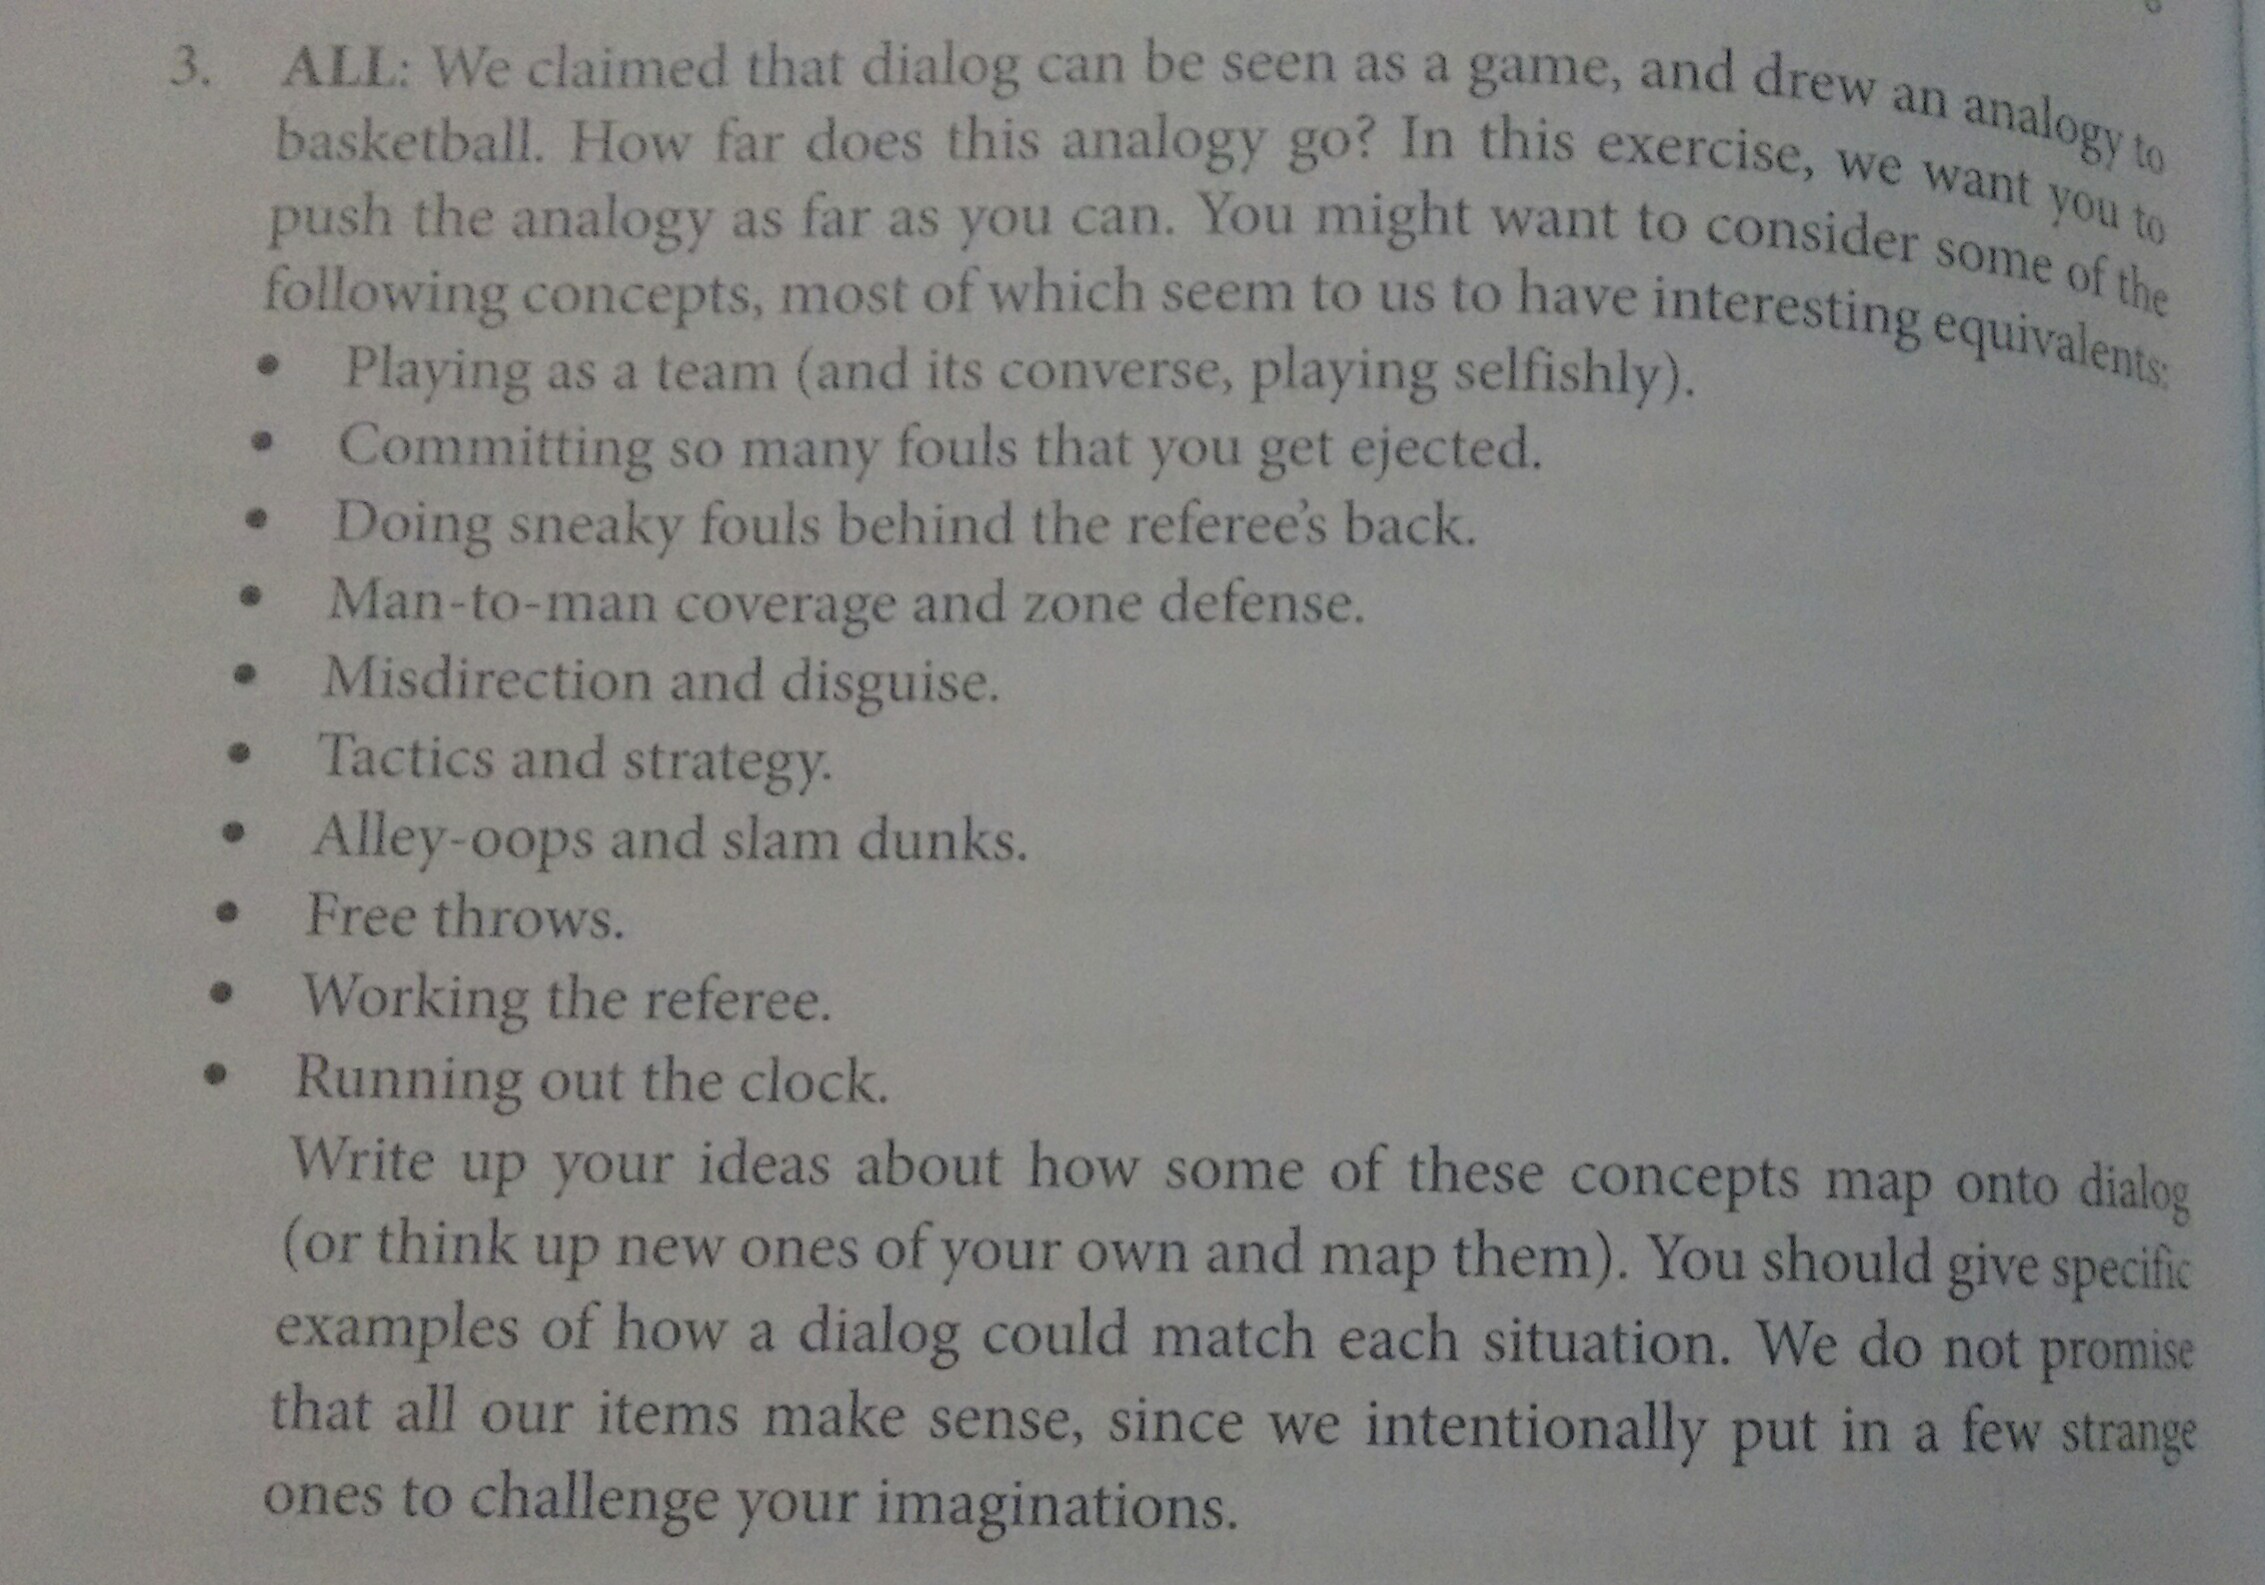
\includegraphics[width=0.9\textwidth]{question.jpg}
\end{frame}

\end{document}
